\documentclass[a4wide]{report}

\usepackage{amsmath}
\usepackage[a4paper, total={7in, 10.2in}]{geometry}
\usepackage{graphicx}
\usepackage[portuguese]{babel}
\usepackage[utf8]{inputenc}

\begin{document}

\noindent
{\bf Lincoln Martins de Oliveira (ES 90693) - Mini-relatório 02 (\today)}

\begin{quote}

\centering

\bf Mini relatório referente ao exercício 2 das aulas 9 e 10

\end{quote}
\vspace{0.5cm}


      Este exercício nos apresenta o metodo dos mínimos quadrados (veja pags 27 e 28 de ~\cite{Metodos}) que utilizamos para realizar
a implementação de um programa que obtem o melhor ajuste de um conjunto de pontos experimentais da forma ($x_{k}$,$y_{k}$) como proposto em ~\cite{roteiro}. 



\begin{quote}

\bf 2) a-

\end{quote}

Neste item foi proposto escrever as expressões analíticas para o sistema de equações obtida pelas derivadas em 
relação aos parâmetros a e b de ~\ref{soma} e fornecer sua solução, isto é, fornecer as formulas de como obtemos os coeficientes 
angular a e linear b da função dos $y_{k}$ e $x_{k}$ experimentais.

\begin{equation}
\centering
S  =   \sum_{k=1}^{n}{(f(x_{k};a,b)- y_{k})^2}
\label{soma}
\end{equation}

Sabemos que $f(x_{k};a,b) = ax + b $, logo substituindo em~\ref{soma} e calculando as derivadas parciais em relação aos parâmetros a e b e igualarmos elas a zero, isto é, 
$\partial S/\partial a = 0$ e $\partial S/\partial b = 0 $,  obtemos as seguintes relações :

\begin{equation}
\centering
\frac{\partial S}{\partial a} = \sum_{k=1}^{n}{(ax_{k} + b - y_{k})x_{k} = 0}
\label{deltaa}
\end{equation}

\begin{equation}
\centering
\frac{\partial S}{\partial b} = \sum_{k=1}^{n}{(ax_{k} + b - y_{k}) = 0}
\label{deltab}
\end{equation}

Fazendo

\begin{equation} 
\centering
A = \sum_{k=1}^{n}{x_{k}}
\label{A}
\end{equation}

\begin{equation}
\centering
B = \sum_{k=1}^{n}{y_{k}}
\label{B}
\end{equation}

\begin{equation}
\centering
C = \sum_{k=1}^{n}{x_{k}^2}
\label{C}
\end{equation}

\begin{equation}
D = \sum_{k=1}^{n}{x_{k}y_{k}}
\label{D}
\end{equation}

Substituindo~\ref{A}~\ref{B}~\ref{C}~\ref{D} nas derivadas parciais~\ref{deltaa}~\ref{deltab} encontramos o seguinte sistema de equações:

\begin{equation}
\centering
aC + bA = D 
\label{sistema1}
\end{equation}

\begin{equation}
\centering
aA + nb = B
\label{sistema1}
\end{equation}

Resolvendo o sistema de equações assima encontramos :

\begin{equation}
\centering
a = \frac{nD - AB}{nC - A^2}
\label{sistema1}
\end{equation}

\begin{equation}
\centering
b = \frac{BC - AD}{nC - A^2}
\label{sistema1}
\end{equation}
 
\begin{quote}

\bf 2) b-

\end{quote}

Neste item utilizamos as equações do item anterior, item a, e implementamos
uma subrotina para calcularmos os coeficiêntes angular e linear ${\bf a}$ e ${\bf b}$ respectivamente 
dos pontos experimentais dados pelo arquivo millikan e atraves do gnuplot calculamos também 
os valores de ${\bf a}$ e ${\bf b}$ para podermos compara-los, o programa corespondente a este 
item esta na pasta $02 b$ nesta pasta também encontra-se o script do gnuplot feito para calcular o fit linear e obter os valores de ${\bf a}$ e ${\bf b}$.

Os valores de ${\bf a}$ e ${\bf b}$ obtidos pelo meu programa foram de :
\begin{equation}
\centering
a =   1.6382785714285741     
\label{CA}
\end{equation}
\begin{equation}
\centering   
b =   2.8535714285681024E-002
\label{CL}
\end{equation}

Os valores de ${\bf a}$ e ${\bf b}$ obtidos pelo fit do gnuplot foram de :

\begin{equation}
\centering
a =   1.63828     
\label{CA}
\end{equation}
\begin{equation}
\centering   
b =   0.0285357
\label{CL}
\end{equation}

Podemos observar que a única coisa que mudou de um método para o outro foi a precisão.
\begin{quote}

\bf 2) c-

\end{quote}

Aqui foi pedido para realizarmos os mesmos calculos do item a considerando o coeficiente
linear sendo zero, isto é, ${\bf b}$ = 0. Deste modo obtemos as seguintes equações:

\begin{equation} 
\centering
\frac{\partial S}{\partial a} = \sum_{k=1}^{n}{(ax_{k} - y_{k})x_{k} = 0}
\label{deltaa2}
\end{equation}
\begin{equation}
\centering
\frac{\partial S}{\partial b} = \sum_{k=1}^{n}{(ax_{k} - y_{k}) = 0}
\label{deltab2}
\end{equation}

utilizando as relações ~\ref{A}~\ref{B}~\ref{C}~\ref{D} obtemos duas relações que nos da o coeficiente angular ${\bf a}$ 

\begin{equation}
\centering
aC - D = 0 \Rightarrow a = \frac{D}{C} 
\label{sistema3}
\end{equation}
\begin{equation}
\centering
aA - B = 0 \Rightarrow a = \frac{B}{A} 
\label{sistema4}
\end{equation}

Podemos utilizar qualquer qualquer uma das duas relações encontradas anteriormente para implementarmos
um programa e obter o coeficiente angular ${\bf a}$, eu escolhi a equação~\ref{sistema3} e implementei 
o programa que se encontra na pasta $02 c$ e o valor de ${\bf a}$ encontrado foi de:

\begin{equation}
\centering
 a =   1.6405260143198093      
\label{CA}
\end{equation}
\begin{quote}

\bf 2) d-

\end{quote}

Aqui foi pedido para criarmos um gráfico incluindo os dados experimentais, a função de ajuste com os parâmetros obtidos
no item b pela minha subrotina, e a função de ajuste utilizando os parâmetros obtidos no item c.

\begin{figure}[h]
\centering
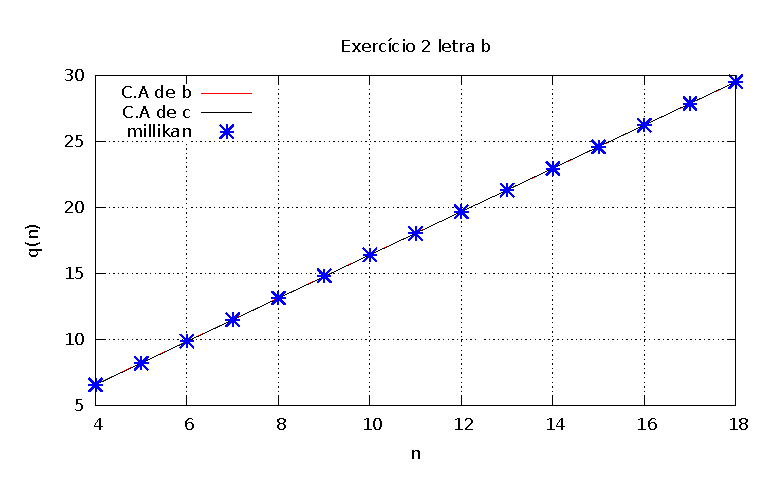
\includegraphics[width=0.6\textwidth]{ex02d}
\caption{O gráfico mostra os pontos experimentais de azul e as retas das regressões obtidas pelos programas das letras b e c 
representadas pelas cores vermelho e preto respectivamente.}
\label{graficoex02d}
\end{figure}

\begin{quote}

\bf 2) e-

\end{quote}


Neste experimento o coeficiente angular ${\bf a}$ repesenta a carga de um único elétron e o coeficiente
linear ${\bf b}$ repesenta algum erro de medida ou a atuação de algum agente esterno durante a realização do
experimento, como não fui eu que o realizou não posso afirmar com certeza quais coisas poderiam alterar o valor das cargas.

O Valor do erro relativo em relação aos itens b e c são respecivamente~\ref{e1} ~\ref{e2} :

\begin{equation}
\centering
 E =   2.2 \%   
\label{e1}
\end{equation}
\begin{equation}
\centering
 E =   2.4 \%   
\label{e2}
\end{equation}



\begin{thebibliography}{99}

\bibitem{Metodos} C. Scherer. Metodos Computacionais da Física (2nd ed.,2010)

\bibitem{roteiro} AULAS 9 E 10: FIS-271 - Física Computacional I

\end{thebibliography}

\end{document}